\chapter{Framework responsive website}
\label{ch:frameworkresponsivewebsite}
\section{Architectuur van de responsive website}
De architectuur van de responsive webapplicatie is het ASP.NET MVC 5 framework van ~\cite{aspnetmvcoverview}.
MVC \footnote{Model View Controller} is een combinatie van design patterns waarbij de business-logica, de user interface en de controllers de belangrijkste
onderdelen zijn. De business-logica bestaat uit domein-objecten die op hun beurt de reële situatie waarbinnen de applicatie
gebruikt wordt, weerspiegelt. Het voornaamste doel van het MVC-framework is een scheiding voorzien tussen het grafische
onderdeel van de toepassing (de schermen), de business logica of model en de controllers die instaan voor het delegeren van gegevens
tussen de views en het model. Schematisch ziet het MVC-framework er als volgt uit:
\begin{figure}[ht!]
\centering
\caption{Schematische voorstelling van het MVC-framework \cite{crossplatformmobiledevelopmentinvisualstudio}}
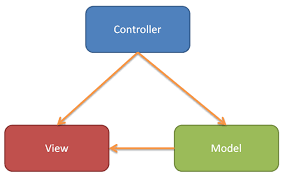
\includegraphics[width=90mm]{./img/mvc.png}
\end{figure}
\section{Voordelen van de gekozen architectuur}
Het ASP.NET MVC 5 framework van ~\cite{aspnetmvcoverview} werd gekozen vanwege volgende voordelen:
\begin{itemize}
  \item Het beheren van complexe applicatie wordt, door de opdeling in Model, View en Controller, eenvoudiger.
  \item Verbeterde ondersteuning voor Test Driven Development \footnote{Test Driven Development is een ontwikkelmethodologie waarbij voorafgaande aan de code eerst de testen geschreven worden. Hierdoor zijn de testen gebaseerd op de oorspronkelijke analyse in plaats van op de geschreven code}
  \item Gecentraliseerde beheer van requests door middel van Front Controller Pattern.
  \item Goede werking voor webapplicaties met grote ontwikkelteams, waarbij de controle over het applicatiegedrag een hoge vereiste is.
\end{itemize}

\section{Nadelen van de gekozen architectuur}
De grootste nadelen van de ASP.NET MVC 5 architectuur zijn volgens ~\cite{hasaspnetcorekilledwebforms} de volgende:
\begin{itemize}
  \item Het moeilijk debuggen van de toepassing in vergelijking met een event-driven variant.
  \item Url's van een ASP.NET MVC 5 applicatie zijn eenvoudiger te begrijpen voor een zoek-robot.
\end{itemize}

\section{Kosten}
Hieronder volgt een overzicht van de voornaamstekosten per fase in de ontwikkeling van de responsive website.
\subsection{Kosten voor de ontwikkeling}
De ontwikkeling van de responsive website is een proces dat niet kostenloos verloopt. Zo moet er een licentie op de ontwikkelomgeving (in dit geval Visual Studio) gekocht worden.
De kosten van deze licentie is afhankelijk van de gekozen. Zo kost een enkele licentie op Visual Studio Professional 2017 499 dollar.

\subsection{Kosten voor testen}
In de testfase zijn er geen kosten verbonden aan de responsive website, aangezien Visual Studio zelf een lokale webserver opzet
voor de hosting van de website. Deze lokale webserver is te bereiken via http://localhost:poortnummer met als poortnummer een
5-cijferig nummer dat vast gekozen is door de ontwikkelomgeving voor de toepassing.
\subsection{Kosten voor publicatie}
Voor de publicatie van de responsive website zijn er volgende optie voor handen:
\begin{itemize}
  \item Men kan kiezen om te hosten op de lokale computer.
  \item Men kan ervoor kiezen om de webapplicatie op een eigen webserver te hosten.
  \item Men kan een externe webserver gebruiken zoals Microsoft Azure.
\end{itemize}
In volgende subsecties worden de kosten zoals electriciteit en koeling van de server buiten beschouwing gelaten omdat deze
mogelijks te grote verschillen opleveren om objectief te kunnen oordelen over de drie publicatiemethoden. Tevens wordt er vanuit
gegaan dat de kosten voor publicatie van de Web api en responsive website gelijk zijn.
%%
\subsubsection{Kosten bij hosting op lokale computer}
De eerste manier van publicatie is het hosten van de webapplicatie op de lokale computer waarop men de responsive website
ontwikkelt. Aan deze manier van publiceren zijn er geen bijkomende kosten verbonden. Het voornaamste nadeel is dat de computer
die de website host, permanent aan dient te staan om de beschikbaarheid te garanderen. Verder is de kost van het installeren
van een webservice minimaal, aangezien die functionaliteit reeds ingebouwd is in de ontwikkelomgeving.
\newpage
\subsubsection{Kosten bij hosting op eigen webserver}
Indien men ervoor kiest om de responsive website op een eigen webserver te hosten, dient men enkel de kosten voor de aankoop en installatie van de webserver in rekening te brengen.
Dit omdat er verder geen kosten zijn voor de hosting van de webserver.

\subsubsection{Kosten bij hosting op externe webserver}
Naast de mogelijkheid om een website zelf te hosten, kan dit ook uitbesteed worden naar een externe service.
Hiervoor worden mogelijks wel kosten voor aangerekend. Bij wijze van voorbeeld vindt u de prijsberekening voor 1 maand Azure hieronder:

  \begin{table}
    \description{Uitgewerkte prijsberekening voor hosting op Azure}
  \begin{tabular}{ | l | l | l | l |}
  \hline
  Omschrijving & Region & Prijscategorie & Prijs (€)
  \\ \hline
  SQL Database (Single Database) & West-Europa & Basis & 4,20
  \\ \hline
  API management & West-Europa & Standaard & 41,30
  \\ \hline
  Support & nvt & nvt & 1,33
  \\ \hline
   & & Totaal &  46,83
  \\ \hline
  \end{tabular}
\end{table}
